\section*{9. The Bootstrap}\label{the-bootstrap}

Let \(X_{1}, \dots, X_{n} \sim F\) be random variables distributed according
to \(F\), and

\[ T_{n} = g(X_{1}, \dots, X_{n})\]

be a \textbf{statistic}, that is, any function of the data. Suppose we
want to know \(\mathbb{V}_F(T_{n})\), the variance of \(T_{n}\).

For example, if \(T_{n} = n^{-1}\sum_{i=1}^{n}X_{i}\) then
\(\mathbb{V}_F(T_{n}) = \sigma^{2}/n\) where
\(\sigma^{2} = \int (x - \mu)^{d}F(x)\) and \(\mu = \int x dF(x)\).

\subsection*{9.1 Simulation}\label{bootstrap:simulation}

Suppose we draw iid samples \(Y_{1}, \dots, Y_B \sim G\). By the law of
large numbers,

\[ \overline{Y}_{n} = \frac{1}{B} \sum_{j=1}^B Y_{j} \; \xrightarrow{\text{P}} \int y dG(y) = \mathbb{E}(Y)\]

as \(B \rightarrow \infty\). So if we draw a large sample from \(G\), we
can use the sample mean to approximate the mean of the distribution.

More generally, if \(h\) is any function with finite mean then, as
\(B \rightarrow \infty\),

\[\frac{1}{B} \sum_{j=1}^B h(Y_{j}) \; \xrightarrow{\text{P}} \int h(y) dG(y) = \mathbb{E}(h(Y))\]

In particular, for functions \(a(Y_{j}) = Y_{j}^{2}\) and \(b(Y_{j}) = Y_{j}\),

\[\frac{1}{B} \sum_{j=1}^B (Y_{j} - \overline{Y}) 
= \frac{1}{B} \sum_{j=1}^B Y_{j}^{2} - \left(\frac{1}{B} \sum_{j=1}^B Y_{j} \right)^{2}
\xrightarrow{\text{P}} \int y^{2} dG(y) - \left( \int y dG(y) \right)^{2} = \mathbb{V}(Y)
\]

So we can use the sample variance of the simulated values to approximate
\(\mathbb{V}(Y)\).

\subsection*{9.2 Bootstrap Variance
Estimation}\label{bootstrap:variance}

To simulate from the distribution of a statistic \(T_{n}\) when the data
is assumed to have distribution \(\hat{F}_{n}\), we simulate
\(X_{1}^*, \dots, X_{n}^*\) from \(\hat{F}_{n}\) and then compute the
statistic over these values, \(T_{n}^* = g(X_{1}^*, \dots, X_{n}^*)\).

\begin{align*}
\text{Real world} \quad      & F         & \Longrightarrow\quad & X_{1}, \dots, X_{n}        & \Longrightarrow & \quad T_{n} = g(X_{1}, \dots, X_{n}) \\
\text{Bootstrap world} \quad & \hat{F}_{n} & \Longrightarrow\quad  & X_{1}^*, \dots, X_{n}^* & \Longrightarrow & \quad T_{n}^* = g(X_{1}^*, \dots, X_{n}^*)
\end{align*}

\textbf{Drawing an observation from \(\hat{F}_{n}\) is equivalent to
drawing one point at random from the original data set.}

\paragraph{Bootstrap Variance
Estimation}\label{bootstrap:variance}

\begin{enumerate}[tightlist,label={\arabic*.}]
\item
  Draw \(X_{1}^*, \dots, X_{n}^* \sim \hat{F}_{n}\).
\item
  Compute \(T_{n}^* = g(X_{1}^*, \dots, X_{n}^*)\).
\item
  Repeat steps 1 and 2, \(B\) times, to get
  \(T_{n, 1}^*, \dots, T_{n, B}^*\).
\item
  Let
\end{enumerate}

\[ v_{\text{boot}} = \frac{1}{B} \sum_{b=1}^B \left( T_{n, b}^* - \frac{1}{B} \sum_{r=1}^B T_{n, r}^* \right)^{2} \]

\subsection*{9.3 Bootstrap Confidence
Intervals}\label{bootstrap-confidence-intervals}

\textbf{Normal Interval}.

\[ T_{n} \pm z_{\alpha/2} \hat{\text{se}}_\text{boot} \]

where \(\hat{\text{se}}_\text{boot}\) is the bootstrap estimate of the
standard error. This is not accurate unless the distribution of \(T_{n}\)
is close to Normal.

\textbf{Pivotal Intervals}.

Let \(\theta = T(F)\), \(\hat{\theta}_{n} = T(\hat{F}_{n})\) and define the
\textbf{pivot} \(R_{n} = \hat{\theta}_{n}  - \theta\). Let
\(\hat{\theta}_{n, 1}^*, \dots, \hat{\theta}_{n, B}^*\) define bootstrap
replications of \(\hat{\theta}_{n}\). Let \(H(r)\) denote the CDF of the
pivot:

\[ H(r) = \mathbb{P}_F(R_{n} \leq r)\]

Define the interval \(C_{n}^* = (a, b)\) where

\[
a = \hat{\theta}_{n} - H^{-1}\left( 1 - \frac{\alpha}{2} \right) 
\quad\text{and}\quad
b = \hat{\theta}_{n} - H^{-1}\left( \frac{\alpha}{2} \right) 
\]

Then,

\begin{align*}
\mathbb{P}(a \leq \theta \leq b) &= \mathbb{P}(a - \hat{\theta}_{n} \leq \theta - \hat{\theta}_{n} \leq b - \hat{\theta}_{n}) \\
&= \mathbb{P}(\hat{\theta}_{n} - b \leq \hat{\theta}_{n} - \theta \leq \hat{\theta}_{n} - a) \\
&= \mathbb{P}(\hat{\theta}_{n} - b \leq R_{n} \leq \hat{\theta}_{n} - a) \\
&= H(\hat{\theta}_{n} - a) - H(\hat{\theta}_{n} - b) \\
&= H\left(H^{-1}\left( 1 - \frac{\alpha}{2} \right) \right) - H\left(H^{-1}\left( \frac{\alpha}{2} \right)\right) \\
&= 1 - \frac{\alpha}{2}  - \frac{\alpha}{2} = 1 - \alpha
\end{align*}

Hence \(C_{n}^*\) is an exact \(1 - \alpha\) confidence interval for
\(\theta\).

Unfortunately, \(a\) and \(b\) depend on the unknown distribution \(H\),
but we can form a bootstrap estimate for it:

\[\hat{H}(r) = \frac{1}{B} \sum_{b=1}^B I(R_{n, b}^* \leq r)\]

where \(R_{n, b}^* = \hat{\theta}_{n, b}^* - \hat{\theta}_{n}\).

Let \(r_\beta^*\) denote the \(\beta\) sample quantile of
\((R_{n, 1}^*, \dots, R_{n, B}^*)\), and let \(\theta_\beta^*\) denote
the \(\beta\) sample quantile of
\((\theta_{n, 1}^*, \dots, \theta_{n, B}^*)\). Note that
\(r_\beta^* = \theta_\beta^* - \hat{\theta}_{n}\). It follows an
approximate \(1 - \alpha\) confidence interval
\(C_{n} = (\hat{a}, \hat{b})\) where

\begin{align*}
\hat{a} 
&= \hat{\theta}_{n} - \hat{H}^{-1}\left(1 - \frac{\alpha}{2}\right) 
&= \hat{\theta}_{n} - r_{1 - \alpha/2}^* 
&= 2\hat{\theta}_{n} - \theta_{1 - \alpha/2}^* \\
\hat{b} 
&= \hat{\theta}_{n} - \hat{H}^{-1}\left(\frac{\alpha}{2}\right) 
&= \hat{\theta}_{n} - r_{\alpha/2}^* 
&= 2\hat{\theta}_{n} - \theta_{\alpha/2}^* 
\end{align*}

The \textbf{\(1 - \alpha\) bootstrap pivotal confidence} is

\[ C_{n} = \left(2 \hat{\theta}_{n} - \hat{\theta}_{1 - \alpha/2}^*, \; 2 \hat{\theta}_{n} - \hat{\theta}_{\alpha/2}^* \right) \]

\textbf{Theorem 9.3}. Under weak conditions on \(T(F)\),

\[ \lim _{n \rightarrow \infty} \mathbb{P}_F\left(T(F) \in C_{n}\right) \rightarrow 1 - \alpha\]

\textbf{Percentile Intervals}.

The \textbf{bootstrap percentile interval} is defined by

\[ C_{n} = \left( \theta_{\alpha/2}^*, \; \theta_{1 - \alpha/2}^*\right) \]

\subsection*{9.5 Technical Appendix}

\paragraph{The Jacknife}\label{the-jacknife}

This method is less computationally expensive than bootstraping, but it
is less general -- it does \emph{not} produce consistent estimates of
the standard errors of the sample quantiles.

Let \(T_{n} = T(X_{1}, \dots, X_{n})\) be a statistic and let \(T_{(-i)}\)
denote the statistic with the \(i\)-th observation removed. Let
\(\overline{T}_{n} = n^{-1} \sum_{i=1}^{n} T_{(-1)}\). The jacknife estimate
of \(\mathbb{V}(T_{n})\) is

\[ v_\text{jack} = \frac{n - 1}{n} \sum_{i=1}^{n} \left(T_{(-i)} - \overline{T}_{n} \right)^{2} \]

and the jacknife estimate of the standard error is
\(\hat{\text{se}}_\text{jack} = \sqrt{v_\text{jack}}\).

Under suitable conditions on \(T\) it can be shown that
\(v_\text{jack} / \mathbb{V}(T_{n}) \xrightarrow{\text{P}} 1\).

\paragraph{Justification for the Percentile
Interval}\label{justification-for-the-percentile-interval}

Suppose there exists a monotone transformation \(U = m(T)\) such that
\(U \sim N(\phi, c^{2})\) where \(\phi = m(\theta)\).

Let \(U_t^* = m(\theta_{n, b}^*)\). Let \(u_\beta^*\) be the sample
quantile of the \(U_b^*\)s. Since a monotone transformation preserves
quantiles, we have that \(u_{\alpha/2}^* = m(\theta_{\alpha/2}^*)\).

Also, since \(U \sim N(\phi, c^{2})\) the \(\alpha/2\) quantile of \(U\)
is \(\phi - z_{\alpha/2}c\). Hence
\(u_{\alpha/2}^* = \phi - z_{\alpha/2}c\). Similarly,
\(u_{1 - \alpha/2}^* = \phi + z_{\alpha/2}c\).

Therefore,

\begin{align*}
\mathbb{P}(\theta_{\alpha/2}^* \leq \theta \leq \theta_{1 - \alpha/2}^*) &=
\mathbb{P}(m(\theta_{\alpha/2}^*) \leq m(\theta) \leq m(\theta_{1 - \alpha/2}^*)) \\
&= \mathbb{P}(u_{\alpha/2}^* \leq \phi \leq u_{1 - \alpha/2}^*) \\
&= \mathbb{P}(U - cz_{\alpha/2} \leq \phi \leq U + cz_{1 - \alpha/2}) \\
&= \mathbb{P}\left(-z_{\alpha/2} \leq \frac{Y - \phi}{c} \leq z_{1 - \alpha/2} \right) \\
&= 1 - \alpha
\end{align*}

\subsection*{9.6 Exercises}

\textbf{Exercise 9.6.1}. Consider the data in example 9.6.

\begin{itemize}[tightlist]
\item
  Find the plug-in estimate of the correlation coefficient.\\
\item
  Estimate the standard error using the bootstrap.\\
\item
  Find a 95\% confidence interval using all three methods.
\end{itemize}

\begin{python}
# Data from example 9.6:

LSAT = [576, 635, 558, 578, 666, 580, 555, 661, 651, 605, 653, 575, 545, 572, 594]
GPA = [3.39, 3.30, 2.81, 3.03, 3.44, 3.07, 3.00, 3.43, 3.36, 3.13, 3.12, 2.74, 2.76, 2.88, 3.96]
\end{python}

\begin{python}
import math
import numpy as np
import pandas as pd
from tqdm import tqdm_{n}otebook

df = pd.DataFrame({'LSAT': LSAT, 'GPA': GPA})
df.plot.scatter(x='LSAT', y='GPA')
\end{python}

\begin{figure}[H]
\centering
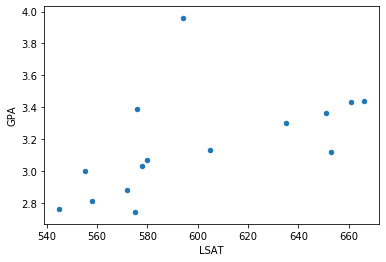
\includegraphics{Figure-09-01}
\end{figure}

\begin{python}
# Plug-in estimates for mean and correlation

X = df['LSAT'].to_{n}umpy()
Y = df['GPA'].to_{n}umpy()

def corr(X, Y):
    mu_x = X.mean()
    mu_y = Y.mean()

    return sum((X - mu_x) * (Y - mu_y)) / math.sqrt(sum((X - mu_x)**2) * sum((Y - mu_y)**2))
  

theta_hat = corr(X, Y)
    
print('Estimated correlation coefficient: %.4f' % corr(X, Y))
\end{python}

\begin{console}
Estimated correlation coefficient: 0.5459
\end{console}

\begin{python}
# Bootstrap for SE of correlation coefficient

nx = len(X)
ny = len(Y)

B = 1000000
t_boot = np.empty(B)
for i in tqdm_{n}otebook(range(B)):
    xx = np.random.choice(X, nx, replace=True)
    yy = np.random.choice(Y, ny, replace=True)
    t_boot[i] = corr(xx, yy)
    
se = t_boot.std()

print('Estimated SE of correlation coefficient: %.4f' % se)
\end{python}


\begin{console}
Estimated SE of correlation coefficient: 0.2674
\end{console}

\begin{python}
# Confidence intervals obtained from bootstrap

from scipy.stats import norm

z = norm.ppf(.975)

normal_conf = (theta_hat - z * se, theta_hat + z * se)
percentile_conf = (np.quantile(t_boot, .025), np.quantile(t_boot, .975))
pivotal_conf = (2*theta_hat - np.quantile(t_boot, 0.975), 2*theta_hat - np.quantile(t_boot, .025))

print('95%% confidence interval (Normal): \t %.3f, %.3f' % normal_conf)
print('95%% confidence interval (percentile): \t %.3f, %.3f' % percentile_conf)
print('95%% confidence interval (pivotal): \t %.3f, %.3f' % pivotal_conf)
\end{python}

\begin{console}
95\% confidence interval (Normal):        0.022, 1.070
95\% confidence interval (percentile):    -0.503, 0.522
95\% confidence interval (pivotal):       0.569, 1.594
\end{console}

\textbf{Exercise 9.6.2}. (Computer Experiment). Conduct a simulation to
compare the four bootstrap confidence interval methods.

Let \(n = 50\) and let \(T(F) = \int (x - \mu)^{3} dF(x) / \sigma^{3}\) be
the skewness. Draw \(Y_{1}, \dots, Y_{n} \sim N(0, 1)\) and set
\(X_{i} = e^{Y_{i}}\), \(i = 1, \dots, n\). Construct the four types of
bootstrap 95\% intervals for \(T(F)\) from the data \(X_{1}, \dots, X_{n}\).
Repeat this whole thing many times and estimate the true coverage of the
four intervals.

\begin{python}
import numpy as np
from tqdm import tqdm_{n}otebook
from scipy.stats import norm

def create_data(n=50):
    y = norm.rvs(size=n)
    return np.exp(y)

def skewness(x):
    n = len(x)
    mu = sum(x) / n
    var = sum((x - mu)**2) / n
    return sum((x - mu)**3 / (n * var**(3/2)))

def bootstrap_values(x, B=10000, show_progress=True):
    n = len(x)
    t_boot = np.empty(B)
    iterable = tqdm_{n}otebook(range(B)) if show_progress else range(B)
    for i in iterable:
        xx = np.random.choice(x, n, replace=True)
        t_boot[i] = skewness(xx)

    return t_boot

def bootstrap_{i}ntervals(theta_hat, t_boot, alpha=0.05):
    se = t_boot.std()
    
    z = norm.ppf(1 - alpha/2)
    q_half_alpha = np.quantile(t_boot, alpha/2)
    q_c_half_alpha = np.quantile(t_boot, 1 - alpha/2)

    normal_conf = (theta_hat - z * se, theta_hat + z * se)
    percentile_conf = (q_half_alpha, q_c_half_alpha)
    pivotal_conf = (2*theta_hat - q_c_half_alpha, 2*theta_hat - q_half_alpha)
    
    return normal_conf, percentile_conf, pivotal_conf
\end{python}

\begin{python}
# Creating the data
x = create_data(n=50)

# Nonparametric Bootstrap
theta_hat = skewness(x)
t_boot = bootstrap_values(x, B=100000)

normal_conf, percentile_conf, pivotal_conf = bootstrap_{i}ntervals(theta_hat, t_boot, alpha=0.05)

print('95%% confidence interval (Normal): \t %.3f, %.3f' % normal_conf)
print('95%% confidence interval (percentile): \t %.3f, %.3f' % percentile_conf)
print('95%% confidence interval (pivotal): \t %.3f, %.3f' % pivotal_conf)
\end{python}

\begin{console}
95\% confidence interval (Normal):        1.032, 2.638
95\% confidence interval (percentile):    1.154, 2.757
95\% confidence interval (pivotal):       0.912, 2.515
\end{console}

\textbf{Note}: parametric bootstrap is only covered in chapter 10. The
below assumes that ``four types of bootstrap'' in the exercise refers to
the 3 types of nonparametric bootstrap covered in chapter 9, plus
parametric bootstrap from chapter 10.

For the parametric bootstrap, assume \(X = e^Y\) where
\(Y \sim N(\mu, \sigma^{2})\). Then

\begin{align*}
\mathbb{E}(X) & = \mathbb{E}(e^Y) = \int_{-\infty}^{\infty} e^y \frac{1}{\sigma \sqrt{2 \pi}} e^{-\frac{1}{2} \left(\frac{y - \mu}{\sigma} \right)^{2}} dy = \frac{1}{\sigma \sqrt{2 \pi}} \int e^{y - \frac{1}{2}\left(\frac{y - \mu}{\sigma}\right)^{2}} dy = e^{\mu + \sigma^{2}/2} \\
\mathbb{E}(X^{2}) &= \mathbb{E}(e^{2Y}) = e^{2\mu + (2\sigma)^{2}/2} = e^{2\mu + 2\sigma^{2}}
\end{align*}

Solving the two equations for the moments we get parameter estimates:

\begin{align*}
\hat{\mu}_Y & = 4 \log \mathbb{E}(X) - \log \mathbb{E}(X^{2}) \\
\hat{\sigma}_Y & = \sqrt{\log \mathbb{E}(X^{2}) - 2 \log \mathbb{E}(X)}
\end{align*}

From these parameter estimates, we can generate bootstrap samples:
sample values for \(Y_{i} ~ N(\hat{\mu}_Y, \hat{\sigma}_Y^{2})\), calculate
\(X_{i} = Y_{i}\), and calculate the statistic \(T(X_{i})\) on each sample
generated this way.

\begin{python}
# Parametric bootstrap
# Assume X = e^Y, Y ~ N(\mu, \sigma^{2})

def estimate_parameters(x):
    log_e_x = np.log(x.mean())
    log_e_x2 = np.log((x**2).mean())
    
    mu_Y_hat = 4 * log_e_x - log_e_x2
    sigma_Y_hat = np.sqrt(log_e_x2 - 2 * log_e_x)
    
    return mu_Y_hat, sigma_Y_hat

def bootstrap_skewness_parametric(mu, sigma, n, B = 10000, show_progress=True):
    t_boot = np.empty(B)
    iterable = tqdm_{n}otebook(range(B)) if show_progress else range(B)
    for i in iterable:
        xx = np.exp(norm.rvs(size=n, loc=n, scale=sigma))
        t_boot[i] = skewness(xx)
        
    return t_boot

def bootstrap_parametric_{i}ntervals(mu, t_boot, alpha=0.05):
    se = t_boot.std()
    z = norm.ppf(1 - alpha/2)
    
    return (theta_hat - z * se, theta_hat + z * se)
\end{python}

\begin{python}
mu_X_hat = x.mean()
mu_Y_hat, sigma_Y_hat = estimate_parameters(x)
t_boot = bootstrap_skewness_parametric(mu_Y_hat, sigma_Y_hat, 50, B=100000)

parametric_{n}ormal_conf = bootstrap_parametric_{i}ntervals(mu_X_hat, t_boot, alpha=0.05)
print('95%% confidence interval (Parametric Normal): \t %.3f, %.3f' % parametric_{n}ormal_conf)
\end{python}

\begin{console}
95\% confidence interval (Parametric Normal):     -0.181, 3.851
\end{console}

\begin{python}
# Repeat nonparametric bootstrap many times
n_experiments = 10

normal_conf = np.empty((n_experiments, 2))
percentile_conf = np.empty((n_experiments, 2))
pivotal_conf = np.empty((n_experiments, 2))

for i in tqdm_{n}otebook(range(n_experiments)):
    theta_hat = skewness(x)
    t_boot_experiment = bootstrap_values(x, B=100000, show_progress=False)
    normal_conf[i], percentile_conf[i], 
                    pivotal_conf[i] = bootstrap_{i}ntervals(theta_hat, t_boot_experiment, alpha=0.05)
\end{python}

\begin{python}
print('Normal confidence lower bound: \t\t mean %.3f, SE %.3f' % 
      (normal_conf[:, 0].mean(), normal_conf[:, 0].std()))
print('Normal confidence upper bound: \t\t mean %.3f, SE %.3f' % 
      (normal_conf[:, 1].mean(), normal_conf[:, 1].std()))

print('Percentile confidence lower bound: \t mean %.3f, SE %.3f' % 
      (percentile_conf[:, 0].mean(), percentile_conf[:, 0].std()))
print('Percentile confidence upper bound: \t mean %.3f, SE %.3f' % 
      (percentile_conf[:, 1].mean(), percentile_conf[:, 1].std()))

print('Pivotal confidence lower bound: \t mean %.3f, SE %.3f' % 
      (pivotal_conf[:, 0].mean(), pivotal_conf[:, 0].std()))
print('Pivotal confidence upper bound: \t mean %.3f, SE %.3f' % 
      (pivotal_conf[:, 1].mean(), pivotal_conf[:, 1].std()))
\end{python}

\begin{console}
Normal confidence lower bound:           mean 1.031, SE 0.001
Normal confidence upper bound:           mean 2.639, SE 0.001
Percentile confidence lower bound:       mean 1.154, SE 0.002
Percentile confidence upper bound:       mean 2.762, SE 0.005
Pivotal confidence lower bound:          mean 0.907, SE 0.005
Pivotal confidence upper bound:          mean 2.515, SE 0.002
\end{console}

\begin{python}
# Repeat parametric bootstrap many times

n_experiments = 10
parametric_{n}ormal_conf = np.empty((n_experiments, 2))

for i in tqdm_{n}otebook(range(n_experiments)):
    mu_X_hat = x.mean()
    mu_Y_hat, sigma_Y_hat = estimate_parameters(x)
    t_boot = bootstrap_skewness_parametric(mu_Y_hat, sigma_Y_hat, 50, B=100000, 
                                                                      show_progress=False)
    parametric_{n}ormal_conf[i] = bootstrap_parametric_{i}ntervals(mu_X_hat, t_boot, alpha=0.05)
\end{python}

\begin{python}
print('Parametric Normal confidence lower bound: \t mean %.3f, SE %.3f' % 
      (parametric_{n}ormal_conf[:, 0].mean(), parametric_{n}ormal_conf[:, 0].std()))
print('Parametric Normal confidence upper bound: \t mean %.3f, SE %.3f' % 
      (parametric_{n}ormal_conf[:, 1].mean(), parametric_{n}ormal_conf[:, 1].std()))
\end{python}

\begin{console}
Parametric Normal confidence lower bound:        mean -0.185, SE 0.003
Parametric Normal confidence upper bound:        mean 3.854, SE 0.003
\end{console}

\textbf{Exercise 9.6.3}. Let \(X_{1}, \dots, X_{n} \sim t_{3}\) where
\(n = 25\). Let \(\theta = T(F) = (q_{.75} - q_{.25})/1.34\) where
\(q_p\) denotes the \(p\)-th quantile. Do a simulation to compare the
coverage and length of the following confidence intervals for
\(\theta\):

\begin{itemize}[tightlist]
\item
  Normal interval with standard error from the bootstrap
\item
  Bootstrap percentile interval
\end{itemize}

Remark: the jacknife does not give a consistent estimator of the
variance of a quantile.

\textbf{Solution}. We will assume that \(t_{3}\) represents a
t-distribution with shape parameter 3.

\begin{python}
import numpy as np
from scipy.stats import t
from tqdm import tqdm_{n}otebook

n = 25
X = t.rvs(3, size=25)
\end{python}

\begin{python}
def T(x):
    return (np.quantile(x, 0.75) - np.quantile(x, 0.25)) / 1.34
\end{python}

\begin{python}
theta_hat = T(X)
\end{python}

\begin{python}
# Run bootstrap

B = 1000000
t_boot = np.empty(B)
for i in tqdm_{n}otebook(range(B)):
    xx = np.random.choice(X, n, replace=True)
    t_boot[i] = T(xx)
    
se_boot = t_boot.std()

alpha = 0.05
z = norm.ppf(1 - alpha/2)
q_half_alpha = np.quantile(t_boot, alpha/2)
q_c_half_alpha = np.quantile(t_boot, 1 - alpha/2)

normal_conf = (theta_hat - z * se_boot, theta_hat + z * se_boot)
percentile_conf = (q_half_alpha, q_c_half_alpha)

print('95%% confidence interval (Normal): \t %.3f, %.3f' % normal_conf)
print('95%% confidence interval (percentile): \t %.3f, %.3f' % percentile_conf)
\end{python}


\begin{console}
95\% confidence interval (Normal):        0.032, 2.089
95\% confidence interval (percentile):    0.605, 2.378
\end{console}

\textbf{Exercise 9.6.4}. Let \(X_{1}, \dots, X_{n}\) be distinct
observations (no ties). Show that there are

\[ \binom{2n - 1}{n}\]

distinct bootstrap samples.

Hint: Imagine putting \(n\) balls into \(n\) buckets.

\textbf{Solution}.

Each bootstrap sample (random draws with replacement) will select
\(a_{i}\) copies of \(X_{i}\), where \(0 \leq a_{i} \leq n\) and
\(\sum_{i=1}^{n} a_{i} = n\), for integer \(a_{i}\). Each bootstrap sample is
uniquely represented by this sequence of variables, and each sequence of
variables uniquely determines a bootstrap sample -- so the number of
distinct bootstrap samples is equal to the number of solutions to this
equation, that is, the number of partitions of \(n\) into \(n\) buckets.

Lets write \(a_{i}\) explicitly in base 1, representing it as \(a_{i}\)
consecutive copies of the digit 1:

\begin{align*}
0_{10} & = \text{empty string}_{1} \\
1_{10} & = 1_{1} \\
2_{10} & = 11_{1} \\
3_{10} & = 111_{1} \\
4_{10} & = 1111_{1} \\
\vdots
\end{align*}

So a solution for

\[a_{1} + a_{2} + \dots + a_{n} = n\]

is uniquely represented by a sequence of \(2n - 1\) symbols, being \(n\)
digits \(1\) and \(n - 1\) plus signs. For example, if \(a_{1} = 3\),
\(a_{2} = 0\), \(a_{3} = 1\), then we write

\[ 111 + + 1 + \dots = n \]

The number of such solutions is then obtained by choosing \(n\) of the
\(2n - 1\) symbols to be digit \(1\) -- that is, \(\binom{2n - 1}{n}\).

\textbf{Exercise 9.6.5}. Let \(X_{1}, \dots, X_{n}\) be distinct
observations (no ties). Let \(X_{1}^*, \dots, X_{n}^*\) denote a bootstrap
sample and let \(\overline{X}_{n}^* = n^{-1}\sum_{i=1}^{n}X_{i}^*\). Find:

\begin{itemize}[tightlist]
\item
  \(\mathbb{E}(\overline{X}_{n}^* | X_{1}, \dots, X_{n})\)
\item
  \(\mathbb{V}(\overline{X}_{n}^* | X_{1}, \dots, X_{n})\)
\item
  \(\mathbb{E}(\overline{X}_{n}^*)\)
\item
  \(\mathbb{V}(\overline{X}_{n}^*)\)
\end{itemize}

\textbf{Solution}.

\textbf{(a)} \begin{align*}
\mathbb{E}(\overline{X}_{n}^* | X_{1}, \dots, X_{n}) &= \mathbb{E}\left(n^{-1}\sum_{i=1}^{n}X_{i}\right) = n^{-1}\sum_{i=1}^{n} \mathbb{E}(X_{i}) = \mathbb{E}(X)
\end{align*}

\textbf{(b)} \begin{align*}
\mathbb{V}(\overline{X}_{n}^* | X_{1}, \dots, X_{n}) & =
\mathbb{E}((\overline{X}_{n}^*)^{2} | X_{1}, \dots, X_{n}) - \mathbb{E}(\overline{X}_{n}^* | X_{1}, \dots, X_{n})^{2} \\
&= \mathbb{E}\left(\left(n^{-1}\sum_{i=1}^{n}X_{i}\right)^{2}\right) - \mathbb{E}\left(n^{-1}\sum_{i=1}^{n}X_{i}\right)^{2} \\
&= n^{-2} \mathbb{E}\left(\sum_{i=1}^{n}X_{i}^{2} + \sum_{i=1}^{n} \sum_{j=1, j \neq i}^{n} X_{i} X_{j}\right) - \mathbb{E}(X)^{2} \\
&= n^{-2} \sum_{i=1}^{n} \mathbb{E}(X_{i}^{2}) + n^{-2} \sum_{i=1}^{n} \sum_{j=1, j \neq i}^{n} \mathbb{E}(X_{i} X_{j}) - \mathbb{E}(X)^{2}  \\
&= n^{-1} (\mathbb{V}(X) + \mathbb{E}(X)^{2}) + n^{-2} \sum_{i=1}^{n} \sum_{j=1, j \neq i}^{n} \mathbb{E}(X_{i}) \mathbb{E}(X_{j}) - \mathbb{E}(X)^{2} \\
&= n^{-1} (\mathbb{V}(X) + \mathbb{E}(X)^{2}) + n^{-1} (n - 1) \mathbb{E}(X)^{2} - \mathbb{E}(X)^{2} \\
&= \frac{1}{n}\mathbb{V}(X)
\end{align*}

\textbf{(c)} \begin{align*}
\mathbb{E}(\overline{X}_{n}^*) &= \mathbb{E}\left(n^{-1} \sum_{i=1}^{n}X_{i}^*\right) = n^{-1} \sum_{i=1}^{n} \mathbb{E}(X_{i}^*) = \mathbb{E}(X)
\end{align*}

\textbf{(d)} \begin{align*}
\mathbb{V}(\overline{X}_{n}^*) &= \mathbb{E}((\overline{X}_{n}^*)^{2}) - \mathbb{E}(\overline{X}_{n}^*)^{2} \\
&= \mathbb{E}\left(\left(n^{-1} \sum_{i=1}^{n}X_{i}^*\right)^{2}\right) - \mathbb{E}(X)^{2} \\
&= n^{-2} \sum_{i=1}^{n}\sum_{j=1}^{n} \mathbb{E}(X_{i}^* X_{j}^*) - \mathbb{E}(X)^{2}
\end{align*}

Now, the same value \(X_{k}\) may have been sampled twice in
\(\mathbb{E}(X_{i}^* X_{j}^*)\). This always happens when \(i = j\), and
this happens with probability \(1 / n\) when \(i \neq j\). Thus,

\begin{align*}
\mathbb{V}(\overline{X}_{n}^*) 
&= n^{-2} \left(\sum_{i=1}^{n} \mathbb{E}(X_{i}^{2}) + \sum_{i=1}^{n} \sum_{j=1, j \neq i}^{n} \left( \frac{1}{n} \mathbb{E}(X_{i}^{2}) + \left(1 - \frac{1}{n}\right)\mathbb{E}(X_{i})\mathbb{E}(X_{j})\right) \right) - \mathbb{E}(X)^{2} \\
&= n^{-1} \mathbb{E}(X^{2}) + n^{-2} (n-1) \mathbb{E}(X^{2}) + n^{-2}(n-1)^{2} E(X)^{2} - \mathbb{E}(X)^{2} \\
&= n^{-2} (2n - 1) \left( \mathbb{E}(X^{2}) - \mathbb{E}(X)^{2} \right) \\
&= \frac{2n - 1}{n^{2}} \mathbb{V}(X)
\end{align*}

\textbf{Exercise 9.6.6}. (Computer Experiment). Let
\(X_{1}, \dots, X_{n} \sim N(\mu, 1)\). Let \(\theta = e^\mu\)and let
\(\hat{\theta} = e^{\overline{X}}\) be the mle. Create a dataset (using
\(\mu = 5\)) consisting of \(n = 100\) observations.

\textbf{(a)} Use the bootstrap to get the \(\text{se}\) and 95\%
confidence interval for \(\theta\).

\textbf{(b)} Plot a histogram of the bootstrap replications for the
parametric and non-parametric bootstraps. These are estimates of the
distribution of \(\hat{\theta}\). Compare this to the true sampling
distribution of \(\hat{\theta}\).

\begin{python}
import numpy as np
import pandas as pd
from scipy.stats import norm
from tqdm import tqdm_{n}otebook

X = norm.rvs(loc=5, scale=1, size=100)
\end{python}

\begin{python}
# Get estimated value

theta_hat = np.exp(X.mean())

# Run nonparametric bootstrap

B = 1000000
t_boot_{n}onparam = np.empty(B)
n = len(X)
for i in tqdm_{n}otebook(range(B)):
    xx = np.random.choice(X, n, replace=True)
    t_boot_{n}onparam[i] = np.exp(xx.mean())
    
se_boot = t_boot_{n}onparam.std()

alpha = 0.05
z = norm.ppf(1 - alpha/2)
normal_conf = (theta_hat - z * se_boot, theta_hat + z * se_boot)

print('95%% confidence interval (Normal): \t %.3f, %.3f' % normal_conf)
\end{python}

\begin{console}
95\% confidence interval (Normal):        104.486, 160.228
\end{console}

\begin{python}
# Run parametric bootstrap

mu_hat = X.mean()
theta_hat = np.exp(mu_hat)

B = 1000000
t_boot_param = np.empty(B)
n = len(X)
for i in tqdm_{n}otebook(range(B)):
    xx = norm.rvs(size=n, loc=mu_hat, scale=1)
    t_boot_param[i] = np.exp(xx.mean())
    
se_boot_param = t_boot_param.std()

alpha = 0.05
z = norm.ppf(1 - alpha/2)
normal_conf_param = (theta_hat - z * se_boot_param, theta_hat + z * se_boot_param)

print('95%% confidence interval (Parametric Normal): \t %.3f, %.3f' % normal_conf_param)
\end{python}


\begin{console}
95\% confidence interval (Parametric Normal):     106.225, 158.490
\end{console}

For the true sampling distribution,

\[ \overline{X} 
= \frac{1}{n} \sum_{i=1}^{n} X_{i} \sim \frac{1}{n} N(n \mu, n) 
= N(\mu, n^{-2})
\]

so the distribution of \(\hat{\theta}\) is the distribution of
\(e^{\overline{X}}\). Its CDF is:

\[
\mathbb{P}\left(\hat{\theta} \leq t\right) 
= \mathbb{P}\left(e^{\overline{X}} \leq t\right) 
= \mathbb{P}\left(\overline{X} \leq \log t\right) 
= F_{\overline{X}}\left(\log t\right)
\]

\begin{python}
import numpy as np
from scipy.stats import norm
import matplotlib.pyplot as plt

bins = np.linspace(50, 250, 500)
\end{python}

\begin{python}
# Generate the CDF for theta, calculate it for each bin, and include the differences between bins

def theta_cdf(x):
    return norm.cdf(np.log(x), loc=5, scale=1/50)

theta_cdf_bins = list(map(theta_cdf, bins))
theta_cdf_bins_delta = np.empty(len(bins))
theta_cdf_bins_delta[0] = 0
theta_cdf_bins_delta[1:] = np.diff(theta_cdf_bins)
\end{python}

\begin{python}
plt.figure(figsize=(12, 8))
plt.hist(t_boot_{n}onparam, bins, label='Nonparametric bootstrap', color='blue', 
         histtype='step', density=True)
plt.hist(t_boot_param, bins, label='Parametric bootstrap', color='red', 
         histtype='step', density=True)
plt.step(bins, theta_cdf_bins_delta, color='green', label='True sampling distribution')
plt.axvline(x=np.exp(5), color='black', label='θ (true parameter)')
plt.legend(loc='upper left')
plt.show()
\end{python}

\begin{figure}[H]
\centering
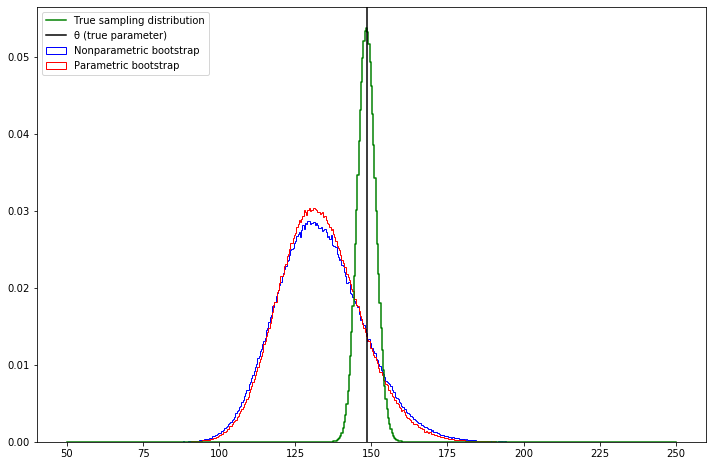
\includegraphics{Figure-09-02}
\end{figure}

\textbf{Exercise 9.6.7}. Let
\(X_{1}, \dots, X_{n} \sim \text{Uniform}(0, \theta)\). The mle is
\(\hat{\theta} = X_\text{max} = \max \{ X_{1}, \dots, X_{n} \}\). Generate a
dataset of size 50 with \(\theta = 1\).

\textbf{(a)} Find the distribution of \(\hat{\theta}\). Compare the true
distribution of \(\hat{\theta}\) to the histograms from the parametric
and nonparametric bootstraps.

\textbf{(b)} This is a case where the nonparametric bootstrap does very
poorly. In fact, we can prove that this is the case. Show that, for
parametric bootstrap \(\mathbb{P}(\hat{\theta}^* = \hat{\theta}) = 0\)
but for the nonparametric
\(\mathbb{P}(\hat{\theta}^* = \hat{\theta}) \approx 0.632\).

Hint: show that
\(\mathbb{P}(\hat{\theta}^* = \hat{\theta}) = 1 - (1 - (1/n))^{n}\) then
take the limit as \(n\) gets large.

\begin{python}
import numpy as np

X = np.random.uniform(low=0, high=1, size=50)
\end{python}

\begin{python}
# Nonparametric bootstrap

theta_hat = X.max()

B = 1000000
t_boot_{n}onparam = np.empty(B)
n = len(X)
for i in tqdm_{n}otebook(range(B)):
    xx = np.random.choice(X, n, replace=True)
    t_boot_{n}onparam[i] = xx.max()
    
se_boot = t_boot_{n}onparam.std()

alpha = 0.05
z = norm.ppf(1 - alpha/2)
normal_conf = (theta_hat - z * se_boot, theta_hat + z * se_boot)

print('95%% confidence interval (Normal): \t %.3f, %.3f' % normal_conf)
\end{python}

\begin{console}
95\% confidence interval (Normal):        0.959, 1.037
\end{console}

\begin{python}
# Run parametric bootstrap

theta_hat = X.max()

B = 1000000
t_boot_param = np.empty(B)
n = len(X)
for i in tqdm_{n}otebook(range(B)):
    xx = np.random.uniform(low=0, high=theta_hat, size=50)
    t_boot_param[i] = xx.max()
    
se_boot_param = t_boot_param.std()

alpha = 0.05
z = norm.ppf(1 - alpha/2)
normal_conf_param = (theta_hat - z * se_boot_param, theta_hat + z * se_boot_param)

print('95%% confidence interval (Parametric Normal): \t %.3f, %.3f' % normal_conf_param)
\end{python}

\begin{console}
95\% confidence interval (Parametric Normal):     0.960, 1.036
\end{console}

For the true sampling distribution,

\[\hat{\theta} = \max \{ X_{1}, \dots X_{n} \}\]

Its CDF is

\[\mathbb{P}(\hat{\theta} \leq x) = \prod_{i=1}^{n} \mathbb{P}(X_{i} \leq x) = F_{\text{Uniform}(0, \theta)}(x)^{n}\]

where

\[F_{\text{Uniform}(0, \theta)}(x) = \begin{cases}
0 & \text{if } x \leq 0 \\
\frac{x}{\theta} & \text{if } 0 < x \leq \theta \\
1 & \text{if } \theta < x
\end{cases}
\]

\begin{python}
bins = np.linspace(0.75, 1.05, 200)
\end{python}

\begin{python}
# Generate the CDF for theta, calculate it for each bin, and include the differences between bins

def theta_cdf(x):
    if x <= 0:
        return 0
    if x >= 1:
        return 1
    return x**50

theta_cdf_bins = list(map(theta_cdf, bins))
theta_cdf_bins_delta = np.empty(len(bins))
theta_cdf_bins_delta[0] = 0
theta_cdf_bins_delta[1:] = np.diff(theta_cdf_bins)
\end{python}

\begin{python}
plt.figure(figsize=(12, 8))
plt.hist(t_boot_{n}onparam, bins, label='Nonparametric bootstrap', color='blue', 
         histtype='step', density=True)
plt.hist(t_boot_param, bins, label='Parametric bootstrap', color='red', 
         histtype='step', density=True)
plt.axvline(x=1, color='black', label='θ (true parameter)')
plt.legend(loc='upper left')
plt.show()
\end{python}

\begin{figure}[H]
\centering
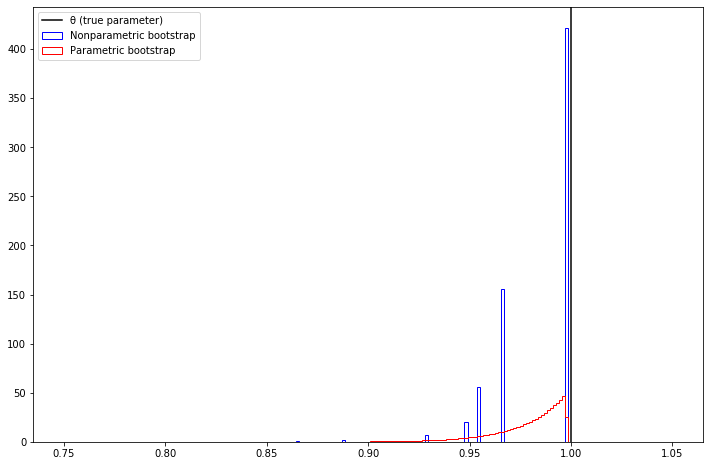
\includegraphics{Figure-09-03}
\end{figure}

\begin{python}
plt.figure(figsize=(12, 8))
plt.step(bins, theta_cdf_bins_delta, color='green', label='True sampling distribution')
plt.axvline(x=1, color='black', label='θ (true parameter)')
plt.legend(loc='upper left')
plt.ylim(0, 0.1)
plt.show()
\end{python}

\begin{figure}[H]
\centering
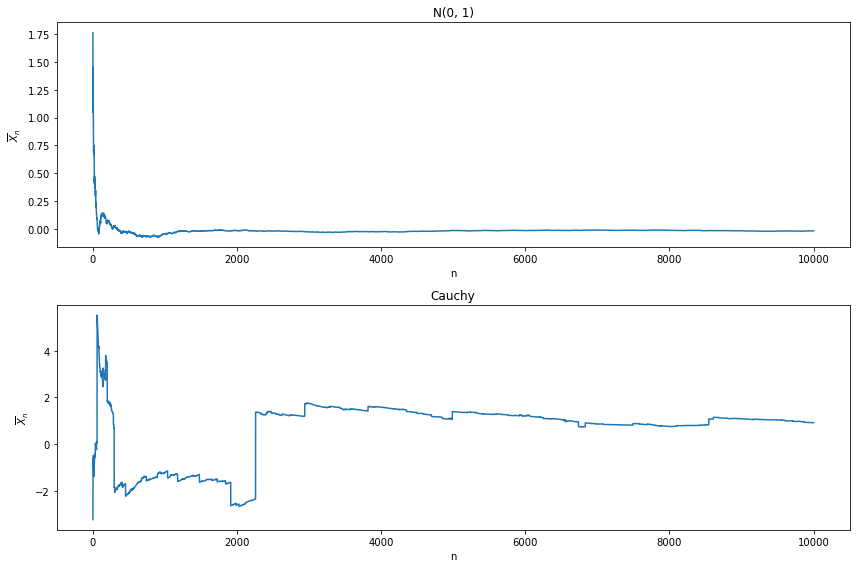
\includegraphics{Figure-04-01}
\end{figure}

\textbf{(b)}

For the parametric bootstrap process, the estimated parameter
\(\hat{\theta}^*\) is used on each \(k\)-th bootstrap sampling
\(\{ X_{k1}, X_{k2}, \dots, X_{kn} \}\). But each variable \(X_{kj}\) is
sampled from \(\text{Uniform}(0, \hat{\theta}^*)\), which is a
continuous distribution -- so the probability of obtaining exactly a
sample at the boundaries is 0, and
\(\mathbb{P}(X_{kj} < \hat{\theta}^*) = 1\). Since the bootstrap
functional of each draw, \(T(F_{n}) = \max(F_{n})\) is the largest drawn
value in each sample, its values will also always be under
\(\hat{\theta}\), thus the estimated parameter via parametric
bootstraping will aywals be under \([\hat{\theta}\), and
\(\mathbb{P}(\hat{\theta}* = \hat{\theta}) = 0\).

For the nonparametric bootstrap process, the estimated parameter
\(\hat{\theta}^*\) is the maximum value with a point mass in the
empirical distribution function \(\hat{F}\). Each bootstrap resample may
or may not include that value when drawing from this sample -- if
\(\max\{X_{1}, \dots, X_{n}\} \in \{X_{k1}, \dots, X_{kn} \}\) then the
estimated functional for that bootstrap sample will be the estimated
parameter \(\hat{\theta}^*\), otherwise it will necessarily be smaller.

Thus, the probability that \(\mathbb{P}(\hat{\theta}* = \hat{\theta})\)
is the probability that the largest element on the original data is
included in a resampling with replacement. That turns out to be one
minus the probability that it never gets included, so,
\(\mathbb{P}(\hat{\theta}* = \hat{\theta}) = 1 - (1 - (1/n))^{n}\). But
\(\lim_{n \rightarrow \infty } (1 + x/n)^{n} = e^x\), so the given
probability goes to \(1 - e^{-1} \approx 0.632\).

\textbf{Exercise 9.6.8}. Let \(T_{n} = \overline{X}_{n}^{2}\),
\(\mu = \mathbb{E}(X_{1})\), \(\alpha_{k} = \int |x - \mu|^{k} dF(x)\) and
\(\hat{\alpha}_{k} = n^{-1} \sum_{i=1}^{n} |X_{i} - \overline{X}_{n}|^{k}\). Show
that

\[v_\text{boot} = \frac{4 \overline{X}_{n}^{2} \hat{\alpha}_{2}}{n} + \frac{4 \overline{X}_{n} \hat{\alpha}_{3}}{n^{2}} + \frac{\hat{\alpha}_{4}}{n^{3}}\]

\textbf{Solution}.

First, we rewrite the sample mean in terms of an expression containing
the central moments. Let
\(S_{n} = n^{-1} \sum_{i=1}^{n} (X_{i} - \overline{X}_{n}) = 0\). Then:

\[ \overline{X}_{n} = S_{n} + \overline{X}_{n} = \frac{1}{n} \sum_{i=1}^{n} (X_{i} - \overline{X}_{n}) + \overline{X}_{n} \]

The bootstrap variance, \(\mathbb{V}\left(\overline{X}_{n}^{2}\right)\), can
be expressed as

\[ \mathbb{V}\left(\overline{X}_{n}^{2}\right) = \mathbb{E}\left(\overline{X}_{n}^{4}\right) - \mathbb{E}\left(\overline{X}_{n}^{2}\right)^{2} \]

Note that \(\overline{X}_{n}\) is the mean of the distribution, and can be
treated as constant when taking expectations.

We now have:

\begin{align*}
\mathbb{E}\left(\overline{X}_{n}^{4}\right) &= \mathbb{E}\left( (S_{n} + \overline{X}_{n})^{4} \right) \\
&= \mathbb{E}\left( S_{n}^{4} + 4 S_{n}^{3} \overline{X}_{n} + 6 S_{n}^{2} \overline{X}_{n}^{2} + 4 S_{n} \overline{X}_{n}^{3} + \overline{X}_{n}^{4} \right) \\
&= \mathbb{E}(S_{n}^{4}) + 4 \overline{X}_{n} \mathbb{E}(S_{n}^{3}) + 6 \overline{X}_{n}^{2} \mathbb{E}(S_{n}^{2}) + 4 \overline{X}_{n}^{3} \mathbb{E}(S_{n}) + \overline{X}_{n}^{4}
\end{align*}

Then, computing the moments of \(S_{n}\),

\begin{align*}
\mathbb{E}(S_{n}) &= 0 \\
\mathbb{E}(S_{n}^{2}) &= \mathbb{E}\left( n^{-2} \left( \sum_{i} X_{i} - \overline{X}_{n} \right)^{2} \right) = \frac{\hat{\alpha}_{2}}{n} \\
\mathbb{E}(S_{n}^{3}) &= \mathbb{E}\left( n^{-3} \left( \sum_{i} X_{i} - \overline{X}_{n} \right)^{3} \right) = \frac{\hat{\alpha}_{3}}{n^{2}} \\
\mathbb{E}(S_{n}^{4}) &= \mathbb{E}\left( n^{-4} \left( \sum_{i} X_{i} - \overline{X}_{n} \right)^{4} + n^{-2}n^{-4} \sum_{i} \sum_{j \neq i} (X_{i} - \overline{X}_{n})^{2} (X_{j} - \overline{X}_{n})^{2} \right) = \frac{\hat{\alpha}_{4} + \hat{\alpha}_{2}^{2}}{n^{3}}
\end{align*}

and finally

\[
\mathbb{E}\left(\overline{X}_{n}^{2}\right)^{2} = \mathbb{E}\left(\overline{X}_{n}^{2} + S_{n}\right)^{2} = \overline{X}_{n}^{4} + 2 \overline{X}_{n}^{2} \frac{\hat{\alpha}_{2}}{n} + \frac{\hat{\alpha}_{2}^{2}}{n^{2}}
\]

Putting everything together,

\begin{align*}
v_\text{boot} &= \mathbb{E}\left( (S_{n} + \overline{X}_{n})^{4} \right) - \mathbb{E}\left(\overline{X}_{n}^{2} + S_{n}\right)^{2} \\
&= \mathbb{E}(S_{n}^{4}) + 4 \overline{X}_{n} \mathbb{E}(S_{n}^{3}) + 6 \overline{X}_{n}^{2} \mathbb{E}(S_{n}^{2}) + 4 \overline{X}_{n}^{3} \mathbb{E}(S_{n}) + \overline{X}_{n}^{4} - \left( \overline{X}_{n}^{4} + 2 \overline{X}_{n}^{2} \frac{\hat{\alpha}_{2}}{n} + \frac{\hat{\alpha}_{2}^{2}}{n^{2}}\right) \\
&= \frac{\hat{\alpha}_{4} + \hat{\alpha}_{2}^{2}}{n^{3}} + 4 \overline{X}_{n} \frac{\hat{\alpha}_{3}}{n^{2}} + 6 \overline{X}_{n}^{2} \frac{\hat{\alpha}_{2}}{n} + 0 + \overline{X}_{n}^{4} - \overline{X}_{n}^{4} - 2 \overline{X}_{n}^{2} \frac{\hat{\alpha}_{2}}{n} - \frac{\hat{\alpha}_{2}^{2}}{n^{2}} \\
&= \frac{4 \overline{X}_{n}^{2} \hat{\alpha}_{2}}{n} + \frac{4 \overline{X}_{n} \hat{\alpha}_{3}}{n^{2}} + \frac{\hat{\alpha}_{4}}{n^{3}}
\end{align*}

Reference and discussion: \url{https://stats.stackexchange.com/q/26082}

